\documentclass[11pt]{article}

\usepackage[margin=1.7cm,top=2.5cm,bottom=2.5cm,legalpaper]{geometry}
\usepackage{enumitem}
\usepackage{tikz,graphicx,wrapfig}
\usepackage{pgfplots}
\usepackage{amsmath}
\usepackage{newtxtext,newtxmath}
\usepackage[document]{ragged2e}
\usepackage[none]{hyphenat}
\usepackage{siunitx}
\usepackage{multicol}
\usepackage{fancyhdr}

\renewcommand{\headrulewidth}{0pt}

\pagestyle{fancy}
\rhead{}
\chead{}
\lhead{}
\lfoot{}\cfoot{-\textsf{\textbf{\thepage}}-}
\rfoot{\textsf{\textbf{GO ON TO THE NEXT PAGE.}}}

\newcommand{\pic}[2]{\includegraphics[width=#1\textwidth]{#2}}
\newcommand{\mb}[1]{\ensuremath\mathbf{#1}}
\sisetup{
  detect-all,
  inter-unit-product =\ensuremath{\cdot{}},
  per-mode=symbol,
  group-separator={,},
}

\begin{document}
\begin{center}
  \textbf{PHYSICS 1\\
    Section I\\
    Time--1 hour 30 minutes\\
    50 Questions
  }
\end{center}

\textbf{Directions:} Each of the questions or incomplete statements below is
followed by five suggested answers or completions. Select the one that is best
in each case and place the letter of your choice in the corresponding box on
the student answer sheet.

\vspace{10pt}
\textbf{Note:} To simplify calculations, you may use $g=\SI{10}{m/s^2}$ in all
problems.

\raggedcolumns
\begin{multicols}{2}
  \textbf{Questions \ref{proj1}--\ref{proj2}} A 10 kg projectile is launched at
  a \ang{60} angle to the ground with a velocity of 200 m/s. Neglect air
  resistance.
  \begin{enumerate}[leftmargin=18pt]
  \item Compare this projectile with a 5 kg projectile launched under the same
    conditions but at a \ang{30} angle. The 5-kg projectile will
    \label{proj1}
    \begin{enumerate}[nosep,leftmargin=18pt,label=(\Alph*)]
    \item go higher up and farther along the ground
    \item go equally high and equally far along the ground
    \item neither go as high nor as far along the ground
    \item not go as high but go equally far along the ground
    \end{enumerate}
    \vspace{.7in}
    
  \item As the launch angle is lowered to \ang{45}, the maximum horizontal
    distance traveled by the projectile will
    \label{proj2}
    \begin{enumerate}[nosep,leftmargin=18pt,label=(\Alph*)]
    \item decrease
    \item increase
    \item remain the same
    \item be impossible to determine without more information
    \end{enumerate}
    \vspace{.7in}
    
    \begin{center}
      \pic{.45}{IMG_20200810_093039201}
    \end{center}
  \item A car with a 500 N driver goes over a hill that has a radius of 50
    meters as shown in the figure above. The velocity of the car is 20 m/s.
    What are the approximate force and direction that the car exerts on the
    driver?
    \begin{enumerate}[nosep,leftmargin=18pt,label=(\Alph*)]
    \item 900 N, up
    \item 400 N, down
    \item 100 N, up
    \item 500 N, up
    \end{enumerate}
    \columnbreak
    
    \begin{center}
      \pic{.3}{falling-blocks}
    \end{center}
  \item Block $Y$ with mass $m_Y$ falls onto and sticks to block $X$, which is
    attached to a vertical spring, as shown in Figure 1. A short time later, as
    shown in Figure 2, the blocks are momentarily at rest. At that moment,
    block $Y$ exerts a force of magnitude $F$ down on block $X$, and block $X$
    exerts a force of magnitude $F$ up on block $Y$. Which of the following
    correctly relates $F_\text{up}$, $F_\text{down}$, and $m_Yg$ at the
    instant shown in Figure 2?
    \begin{enumerate}[nosep,leftmargin=18pt,label=(\Alph*)]
    \item$\left(F_\mathrm{up}=F_\mathrm{down}\right)>m_Yg$
    \item$\left(F_\mathrm{up}=m_Y\right)>F_\mathrm{down}$
    \item$m_Yg > F_\mathrm{up} > F_\mathrm{down}$
    \item$F_\mathrm{up}=F_\mathrm{down}=m_Yg$
    \end{enumerate}
    \vspace{.7in}
    
    \begin{center}
      \pic{.4}{downpour}
    \end{center}
  \item An open cart on a level surface is rolling without frictional loss
    through a vertical downpour of rain, as shown above. As the cart rolls,
    an appreciable amount of rainwater accumulates in the cart. The speed of
    the cart will
    \begin{enumerate}[nosep,leftmargin=18pt,label=(\Alph*)]
    \item increase because of conservation of momentum
    \item increase because of conservation of energy
    \item decrease because of conservation of momentum
    \item decrease because of conservation of energy
    \end{enumerate}
    \columnbreak

    
    \begin{center}
      \pic{.4}{rough-ramp}
    \end{center}
  \item A block is released from rest and slides down a ramp. The surface of
    the ramp has three rough sections where the friction between the surface
    and the block is not negligible, as shown by the shaded regions above.
    Measuring which of the following will allow for the best estimate of the
    block's instantaneous acceleration when the block is at the midpoint of the
    ramp?
    \begin{enumerate}[nosep,leftmargin=18pt,label=(\Alph*)]
    \item The total distance traveled by the block and the total elapsed time
    \item The final speed of the block and the total elapsed time
    \item The distance between points just before and just after the midpoint
      and the time it takes the block to travel between them
    \item The speed of the block at points just before and just after the
      midpoint and the time it takes the block to travel between them
    \end{enumerate}
    \vspace{.7in}
    
  \item A solid metal ball and a hollow plastic ball of the same external
    radius are released from a large vacuum chamber. When each has fallen 1 m,
    they both have the same
    \begin{enumerate}[nosep,leftmargin=18pt,label=(\Alph*)]
    \item inertial
    \item speed
    \item momentum
    \item kinetic energy
    \item change in potential energy
    \end{enumerate}
    \vspace{.75in}
    
    \begin{center}
      \pic{.4}{spring-block}
    \end{center}
  \item A block is held at rest against a compressed spring at point $A$ at the
    top of a frictionless track of height $h$, as shown above. The block is
    released, loses contact with the spring at point $B$, and slides along the
    track until it passes point $C$, also at height $h$. How do the potential
    energy U of the block-Earth system and the kinetic energy $K$ of the block
    at point $C$ compare with those at point $A$?

    \begin{tabular}{ccc}
      & Potential Energy of & Kinetic Energy \\ 
      & Block-Earth System  & of Block \\
      \hline
      (A) & $U_C=U_A$ & $K_C=K_A$ \\
      (B) & $U_C=U_A$ & $K_C>K_A$ \\
      (C) & $U_C>U_A$ & $K_C=K_A$ \\
      (D) & $U_C>U_A$ & $K_C>K_A$ \\
    \end{tabular}

    \begin{center}
      \pic{.3}{fixed-end}
    \end{center}
  \item One end of a horizontal string is fixed to a wall. A transverse wave
    pulse is generated at the other end, moves toward the wall as shown above,
    and is reflected at the wall. Properties of the reflected pulse include
    which of the following?
    \begin{enumerate}[noitemsep,topsep=0pt,leftmargin=18pt,label={\Roman*.}]
    \item It has greater speed than that of the incident pulse.
    \item It has greater amplitude than that of the incident pulse.
    \item It is on the opposite side of the string from the incident pulse.
    \end{enumerate}
    \begin{enumerate}[nosep,leftmargin=18pt,label=(\Alph*)]
    \item I only
    \item III only
    \item I and II only
    \item I and III only
    \item I, II and III
    \end{enumerate}
    \vspace{.7in}
    
    \begin{center}
      \pic{.4}{impulses}
    \end{center}
  \item Objects $X$ and $Y$ are constrained to move along a straight line. The
    graphs above show the net force exerted along that line on each of the
    objects as functions of time. Which of the following correctly ranks the
    change in momentum $\Delta p$ of the objects?
    \begin{enumerate}[noitemsep,topsep=0pt,leftmargin=18pt,label=(\Alph*)]
    \item $\Delta p_X < \Delta p_Y$
    \item $\Delta p_X = \Delta p_Y$ 
    \item $\Delta p_X > \Delta p_Y$
    \item The ranking cannot be determined without knowing the masses of the
      objects.
    \end{enumerate}
  \end{enumerate}
  \columnbreak
  
  \begin{center}
    \pic{.5}{circular-arc}
  \end{center}
  \textbf{Questions \ref{first}--\ref{last}} The figures above show a small
  block of mass 0.20 kg on a track in the shape of a circular arc. The block is
  released from rest at a height $H$ above the floor, as shown in Figure 1. The
  block slides along the track with negligible friction and leaves it at a
  height of 0.40 m above the floor and a speed of 3.0 m/s at a \ang{30} angle,
  as shown in Figure 2.

  \begin{enumerate}[leftmargin=18pt,resume]
  \item The height $H$ is most nearly
    \begin{enumerate}[noitemsep,topsep=0pt,leftmargin=18pt,label=(\Alph*)]
    \item 0.45 m
    \item 0.51 m
    \item 0.86 m
    \item 1.7 m
    \end{enumerate}
    \label{first}
    
  \item The magnitude of the gravitational force exerted on the block is $F_g$,
    and the magnitude of the normal force exerted by the track on the block is
    $F_n$. Which of the following correctly compares the magnitudes of these
    two forces when the block is at the lowest point on the track?
    \begin{enumerate}[nosep,leftmargin=18pt,label=(\Alph*)]
    \item $F_n>F_g$
    \item $F_n=F_g$
    \item $F_n<F_g$
    \item The magnitudes cannot be compared without knowing the radius of the
      arc of the track.
    \end{enumerate}
    \vspace{.7in}
    
  \item After the block leaves the track, what is the block's speed when it
    reaches the highest point of its motion?
    \begin{enumerate}[nosep,leftmargin=18pt,label=(\Alph*)]
    \item 0
    \item 1.5 m/s
    \item 2.6 m/s
    \item 3.0 m/s
    \end{enumerate}
    \label{last}
    \vspace{.7in}
    
  \item Two satellites are in circular orbits around Earth. Satellite 1 has
    mass $m_0$ and an orbital radius of $2R_E$, where $R_E$ is the radius of
    Earth. Satellite 2 has mass $2m_0$ and an orbital radius of $3R_E$. Which
    of the following correctly compares the magnitude $F$ of the force exerted
    by Earth on each satellite and the speed $v$ of each satellite?

    \begin{tabular}{ccc}
      & Force & Speed\\
      \hline
      (A)  & $F_1 > F_2$ & $v_1 > v_2$ \\
      (B)  & $F_1 > F_2$ & $v_2 > v_1$ \\
      (C)  & $F_2 > F_1$ & $v_1 > v_2$ \\
      (D)  & $F_2 > F_1$ & $v_2 > v_1$
    \end{tabular}    
    \columnbreak
    
    \begin{center}
      \pic{.1}{push}
    \end{center}
  \item A person exerts an upward force on a box, as shown above. The box may be
    moving upward, downward, or not at all while the person exerts the upward
    force. For which of the following motions of the box is the work done by the
    person on the box correctly indicated?

    \begin{tabular}{cll}
      & Motion of Box & Work Done by\\
      &               & Person on Box \\
      \hline
      (A) & No motion                      & Positive \\
      (B) & Upward, decreasing speed   & Negative \\
      (C) & Downward, constant speed   & Zero     \\
      (D) & Downward, increasing speed & Negative
    \end{tabular}
    \vspace{.7in}
    
    \begin{center}
      \pic{.48}{car-collision}
    \end{center}
  \item In the setup shown above, a student uses motion detector 1 to measure
    the speed $v_i$ of a cart with mass m before it collides with and sticks to
    a stationary cart with mass $M$. Motion detector 2 measures the speed $v_f$
    of the carts after the collision. The student repeats the experiment
    several times using different values of $v_i$ and creates a graph of $v_f$
    as a function of $v_i$. The slope of this graph is most nearly equal to
    \begin{enumerate}[noitemsep,topsep=0pt,leftmargin=18pt,label=(\Alph*)]
    \item$\displaystyle\frac{m}{M}$
    \item$\displaystyle\frac{m}{M+m}$
    \item$\displaystyle\frac{M-m}{M+m}$
    \item$\displaystyle\sqrt{\frac{m}{M+m}}$
    \end{enumerate}
    \columnbreak
    
  \item Three forces at on an object. If the object is in translational
    equilibrium, which of the following must be true?
    \begin{enumerate}[noitemsep,topsep=0pt,leftmargin=18pt,label={\Roman*.}]
    \item The vector sum of the three forces must be equal
    \item The magnitudes of the three forces must be equal
    \item All three forces must be parallel
    \end{enumerate}
    \begin{enumerate}[noitemsep,topsep=0pt,leftmargin=18pt,label=(\Alph*)]
    \item I only
    \item II only
    \item I and III only
    \item II and III only
    \item I, II and III
    \end{enumerate}
    \vspace{.7in}
    
    \begin{center}
      \pic{.45}{standing-wave}
    \end{center}
  \item A standing wave is produced on a horizontal string of length 3 m that
    is fixed at both ends. The graph above shows the amplitude A of the
    vertical oscillations of points on the string as a function of the distance
    $x$ from one end of the string. For any point on the string, the amplitude
    is the absolute value of the maximum displacement of that point from its
    equilibrium position. The wavelength of the standing wave is
    \begin{enumerate}[nosep,leftmargin=18pt,label=(\Alph*)]
    \item 1.0 m
    \item 1.5 m
    \item 2.0 m
    \item 3.0 m
    \end{enumerate}

    \begin{center}
      \pic{.35}{two-masses}
    \end{center}
  \item A block of mass 3.0 kg is hung from a spring, causing it to stretch 12
    cm at equilibrium, as shown above. The 3.0 block is then replaced by a 4.0
    kg block, and the new block is released from the positive shown above, at
    which the spring is unstretched. How far will the 4.0 kg block fall before
    its direction is reversed?
    \begin{enumerate}[nosep,leftmargin=18pt,label=(\Alph*)]
    \item 9 cm
    \item 18 cm
    \item 24 cm
    \item 32 cm
    \item 48 cm
    \end{enumerate}
    \columnbreak
    
  \item Which of the following statements about a satellite in an elliptical
    orbit around Earth are correct? Select two answers.
    \begin{enumerate}[nosep,leftmargin=18pt,label=(\Alph*)]
    \item The satellite's kinetic energy is constant throughout the orbit.
    \item The satellite's angular momentum about the center of mass of the
      satellite-Earth system is constant throughout the orbit.
    \item The magnitude of the satellite's linear momentum is constant
      throughout the orbit.
    \item The gravitational potential energy of the Earth-satellite system is
      greatest at the satellite's farthest point from Earth.
    \end{enumerate}
    \vspace{.7in}
    
  \item Which of the following can be used as evidence for the claim that the
    energy carried by a mechanical wave increases with the amplitude of the
    wave? Select two answers.
    \begin{enumerate}[noitemsep,topsep=0pt,leftmargin=18pt,label=(\Alph*)]
    \item A person does not move when a small ocean wave passes by but is pushed
      over by a higher wave.
    \item A high-pitched sound may cause more discomfort to a person's ear than
      a low-pitched sound does.
    \item The interference of two waves of amplitude $A_0$ may result in an
      amplitude that is either larger or smaller than $A_0$.
    \item A wave pulse on a string is larger or smaller, depending on how far
      the person creating the pulse moves the end of the string.
    \end{enumerate}
    \vspace{.7in}
    
    \begin{center}
      \pic{.4}{rod}
    \end{center}
  \item A rod on a horizontal tabletop is pivoted at one end and is free to
    rotate without friction about a vertical axis, as shown above. A force
    $\mb{F}$ is applied at the other end, at an angle $\theta$ to the rod. If
    $\mb{F}$ were to be applied for the rod, at what distance from the axis
    should it be applied in order to produce the same torque?
    \begin{enumerate}[noitemsep,topsep=0pt,leftmargin=18pt,label=(\Alph*)]
    \item$L\sin\theta$
    \item$L\cos\theta$
    \item$L$
    \item$L\tan\theta$
    \item$\sqrt{2}L$
    \end{enumerate}
    \columnbreak
    
    \begin{center}
      \begin{tikzpicture}[scale=2]
        \draw[thick,->](0,0)--(0,1)node[midway,left]{$mV$};
        \draw[thick,->](0,0)--(1,0)node[midway,below]{$mV$};
      \end{tikzpicture}
    \end{center}
  \item A stationary object explodes, breaking into three pieces of masses $m$,
    $m$ and $3m$. The two pieces of mass $m$ move off at right angles to each
    other with the same magnitude of momentum $mV$, as shown in the diagram
    above. What are the magnitude and direction of the velocity of the piece
    having mass $3m$?

    \begin{tabular}{ccc}
      & Magnitude & Direction \\
      \hline
      (A) & $\displaystyle\frac{V}{\sqrt{3}}$ & $\nearrow$ \\
      (B) & $\displaystyle\frac{V}{\sqrt{3}}$ & $\swarrow$ \\
      (C) & $\displaystyle\frac{\sqrt{2}V}{3}$ & $\nearrow$ \\
      (D) & $\displaystyle\frac{\sqrt{2}V}{3}$ & $\swarrow$ \\
      (E) & $\displaystyle\sqrt{2}V$ & $\swarrow$ \\
    \end{tabular}
    \vspace{.7in}
    
  \item An old record player could bring a disk up to 45 rpm speed in less than
    a second. If the same size disk can also be brought up to a speed of 75 rpm
    in about the same amount of time on another player, compare the two torques.
    \begin{enumerate}[nosep,leftmargin=18pt,label=(\Alph*)]
    \item The torques would be the same as the amount of rotational inertia of
      the two disks are the same.
    \item The torques would be the same because of the conservation of angular
      momentum.
    \item The torque would be larger in the second case as it requires a
      greater angular acceleration.
    \item The torque would be larger in the second case as it entails both a
      larger force and a larger lever arm.
    \end{enumerate}
    \columnbreak
    
    \begin{center}
      \pic{.25}{rim}
    \end{center}
  \item A wheel of radius $R$ and negligible mass is mounted on a horizontal
    frictionless axle so that the wheel is in a vertical plane. Three small
    objects having masses $m$, $M$ and $2M$, respectively, are mounted on the
    rim of the wheel, as shown above. If the system is in static equilibrium,
    what is the value of $m$ in terms of $M$?
    \begin{enumerate}[noitemsep,topsep=0pt,leftmargin=18pt,label=(\Alph*)]
    \item$\displaystyle\frac{M}{2}$
    \item$M$
    \item$\displaystyle\frac{3M}{2}$
    \item$2M$
    \item$\displaystyle\frac{5M}{2}$
    \end{enumerate}

  \item A 2 kg object moves in a circle of radius 4 m at a constant speed of
    3 m/s. A net force of 4.5 N acts on the object. What is the angular
    momentum of the object with respect to an axis perpendicular the circle
    and through its center?
    \begin{enumerate}[nosep,leftmargin=18pt,label=(\Alph*)]
    \item\SI{9}{N.m/kg}
    \item\SI{12}{m^2/s}
    \item\SI{13.5}{kg.m^2/s^2}
    \item\SI{18}{N.m/kg}
    \item\SI{24}{kg.m^2/s}
    \end{enumerate}
    \vspace{.7in}
    
    \begin{center}
      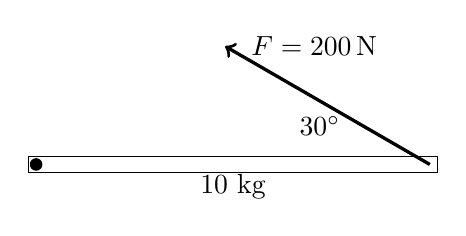
\begin{tikzpicture}
        \fill(-5,0) circle(.08);
        \draw(-5.1,-.1) rectangle (.1,.1)
        node[midway,below]{10 kg};
        \draw[very thick,->,rotate=-30](0,0)--(-3,0)
        node[midway,below]{\ang{30}\;\;}
        node[pos=1,right]{\;\;$F=\SI{200}{\newton}$};
      \end{tikzpicture}
    \end{center}
    
  \item What is the net torque acting on the pivot supporting a 10 kg beam 2
    meters long as shown above?
    \begin{enumerate}[nosep,leftmargin=18pt,label=(\Alph*)]
    \item\SI{198}{\newton.\metre}
    \item\SI{-198}{\newton.\metre}
    \item\SI{-102}{\newton.\metre}
    \item\SI{102}{\newton.\metre}
    \end{enumerate}
    \columnbreak
  \end{enumerate}   
  
  \textbf{Question \ref{mass1}--\ref{mass2}} A 0.4 kg mass is oscillating on a
  spring that has a force constant of $k=\SI{1000}{\newton\per\metre}$.
  \begin{enumerate}[leftmargin=18pt,resume]
  \item Which of the following measurements would allow you to determine the
    maximum velocity experienced by the mass?
    \label{mass1}
    \begin{enumerate}[noitemsep,topsep=0pt,leftmargin=18pt,label=(\Alph*)]
    \item No additional information is required.
    \item Minimum velocity
    \item Maximum acceleration
    \item None of these would allow you to determine maximum velocity
    \end{enumerate}
    \columnbreak
    
  \item Which of the following statements concerning the oscillatory motion
    described is correct? (All statements refer to magnitudes.)
    \label{mass2}
    \begin{enumerate}[noitemsep,topsep=0pt,leftmargin=18pt,label=(\Alph*)]
    \item The maximum velocity and maximum acceleration occurs at the same time.
    \item The maximum velocity occurs when the acceleration is a minimum.
    \item The velocity is always directly proportional to the displacement.
    \item The maximum velocity occurs when the displacement is a maximum.
    \end{enumerate}
  \end{enumerate}
\end{multicols}

\vspace{.7in}
\begin{center}
  \pic{.3}{disks}
  
  \begin{minipage}{.6\textwidth}
    \begin{enumerate}[leftmargin=18pt,start=31]
    \item Cylindrical disk $A$ is rotating freely about an axis when an
      identical disk $B$ that is not rotating is dropped directly on top of disk
      $A$. If the two disks stick together, how does the total angular momentum
      and total kinetic energy of the two-disk system after the disks are stuck
      together compare to that of the system before disk $B$ was dropped?
  
      \begin{tabular}{cll}
        & Total Angular Momentum & Total Kinetic Energy\\
        \hline
        (A) & Remains the same & One-half its original value\\
        (B) & Remains the same & One-fourth its original value\\
        (C) & One-half its original value & One-half its original value\\
        (D) & One-half its original value & One-fourth its original value
      \end{tabular}
    \end{enumerate}
  \end{minipage}
\end{center}
\vspace{\stretch{1}}
\begin{center}
  \textbf{\LARGE S T O P}
  
  \vspace{.3in}END OF SECTION I

  \vspace{.3in}IF YOU FINISH BEFORE TIME IS CALLED, YOU MAY\\
  CHECK YOUR WORK ON THIS SECTION

  \vspace{.3in}DO NOT GO ON TO SECTION II UNTIL YOU ARE TOLD TO DO SO
\end{center}
\end{document}
